\documentclass[12pt]{article}
%\usepackage{fullpage}
\usepackage{epic}
\usepackage{eepic}
\usepackage{paralist}
\usepackage{graphicx}
\usepackage{algorithm,algorithmic}
\usepackage{tikz}
\usepackage{xcolor,colortbl}
\usepackage{amsmath, amssymb}

%%%%%%%%%%%%%%%%%%%%%%%%%%%%%%%%%%%%%%%%%%%%%%%%%%%%%%%%%%%%%%%%
% This is FULLPAGE.STY by H.Partl, Version 2 as of 15 Dec 1988.
% Document Style Option to fill the paper just like Plain TeX.

\typeout{Style Option FULLPAGE Version 2 as of 15 Dec 1988}

\topmargin 0pt
\advance \topmargin by -\headheight
\advance \topmargin by -\headsep

\textheight 8.9in

\oddsidemargin 0pt
\evensidemargin \oddsidemargin
\marginparwidth 0.5in

\textwidth 6.5in
%%%%%%%%%%%%%%%%%%%%%%%%%%%%%%%%%%%%%%%%%%%%%%%%%%%%%%%%%%%%%%%%

\pagestyle{empty}
\setlength{\oddsidemargin}{0in}
\setlength{\topmargin}{-0.8in}
\setlength{\textwidth}{6.8in}
\setlength{\textheight}{9.5in}

\setcounter{secnumdepth}{0}

\setlength{\parindent}{0in}
\addtolength{\parskip}{0.2cm}
\setlength{\fboxrule}{.5mm}\setlength{\fboxsep}{1.2mm}
\newlength{\boxlength}\setlength{\boxlength}{\textwidth}
\addtolength{\boxlength}{-4mm}

\newcommand{\algosolutionbox}[2]{
  \begin{center}
    \framebox{\parbox{\boxlength}{
        \textbf{CS 5722, Fall 2014} \hfill \textbf{#1}\\
        #2
      }}
  \end{center}}

\begin{document}

\algosolutionbox{Homework 7}{
  % TODO: fill in your own name, netID, and collaborators
  Group: Michael Jalkio, Kevin Li, Daniel Sperling\\
  NetIDs: mrj77, kyl27, dhs252
}

\section{i}
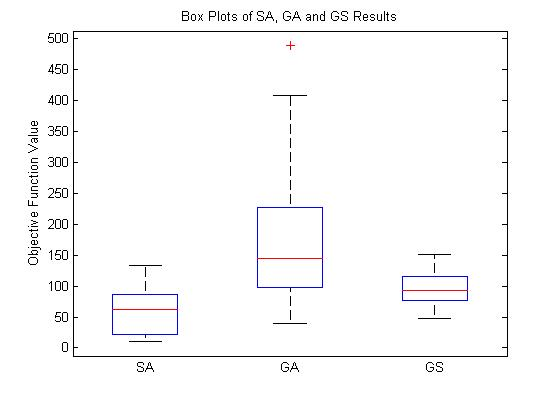
\includegraphics{boxplot}\\
Simulated annealing performs best on average. Greedy search performs second
best, but with a lower variance. The genetic algorithm performs worst, with a
very high variance. There was one outlier in the genetic algorithm, with a
value of 488.83. The best algorithm is simulated annealing, with the lowest
average objective value and a reasonable variance.

\section{ii}
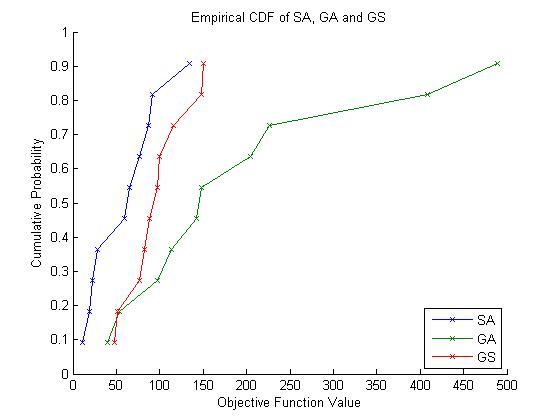
\includegraphics[scale=0.6]{cdf}\\
The simulated annealing algorithm performs best, and stochastically dominates
both greedy search and the genetic algorithm.


\section{iii}
The null hypothesis for each pair is that the mean value of the two search heuristics is the same.

\subsection{SA/GA}
Statistics: T Statistic: -2.736028\\
P value for Two Sided: 0.020504\\
P value for One Sided: 0.010252\\

For comparison at $\alpha = 0.05$, $t_{\alpha/2,v} = 2.220195$, $t_{\alpha, v}  = 1.807620$. As $t < -t_{\alpha/2,v}$, we reject the null hypothesis and accept that the two mean values are the same. Then, since $t <= -t_{\alpha, v}$, we can accept the alternate hypothesis that $\mu_x - \mu_y < \Delta_0$, indicating that the mean of SA is statistically significantly less than the mean of GA.


\subsection{SA/GS}
Statistics: T Statistic: -2.176592\\
P value for Two Sided: 0.043283\\
P value for One Sided: 0.021642\\

For comparison at $\alpha = 0.05$, $t_{\alpha/2,v} = 2.103228$, $t_{\alpha, v}  = 1.735502$. As $t < -t_{\alpha/2,v}$, we reject the null hypothesis and accept that the two mean values are the same. Then, since $t <= -t_{\alpha, v}$, we can accept the alternate hypothesis that $\mu_x - \mu_y < \Delta_0$, indicating that the mean of SA is statistically significantly less than the mean of GS.

\subsection{GA/GS}
Statistics: T Statistic: 2.003192\\
P value for Two Sided: 0.073018\\
P value for One Sided: 0.036509\\

For comparison at $\alpha = 0.05$, $t_{\alpha/2,v} = 2.228346$, $t_{\alpha, v}  = 1.812587$. Since $t \nless -t_{\alpha/2,v}$ and $t \ngtr t_{\alpha/2,v}$, we cannot reject the null hypothesis that the means of the GA and GS are statistically significantly the same.


\section{iv}
Yes; we would use the paired t-test, as it is a more accurate test for algorithms using the same number of runs and identical initial solutions as is the case here. The null hypothesis is the same, that the mean found from the search performed by each of the two search heuristics, SA and GS, is the same. \\

Statistics: T Statistic: -2.415644\\ 
P value for Two Sided: 0.038887\\
P value for One Sided: 0.019444\\

The results here are the same as in section iii, but slightly stronger. The p-value is lower for two sided, 0.0389 compared to 0.043283, indicating a higher level of confidence that the mean values are different. At $\alpha = 0.05$, $t_{\alpha/2,v} = 2.262157$, $t_{\alpha, v}  = 1.833113$. As $t < -t_{\alpha/2,v}$, we reject the null hypothesis and accept that the two mean values are the same. Then, since $t <= -t_{\alpha, v}$, we can accept the alternate hypothesis that $\mu_x - \mu_y < \Delta_0$, indicating that the mean of SA is statistically significantly less than the mean of GS.

\section{v}
The null hypothesis for each pair is that the difference between the means of the two heuristics is zero.
\subsection{SA/GA}
Statistics: Z Statistic: -2.721344\\
P value for Two Sided: 0.003251\\
P value for One Sided: 0.006502\\

For comparison at $\alpha = 0.05$, $z_{\alpha/2}=1.959964$ and $z_{\alpha}=1.644854$.  As $z < -z_{\alpha/2}$, we reject the null hypothesis that the difference between the means of the two heuristics is zero and accept the alternative hypothesis that the difference is some other value.  Because $z<-z_\alpha$ we can also accept the alternate hypothesis that $\mu_X - \mu_Y < \Delta_0$, indicating that the mean of SA is statistically significantly less than the mean of GA.  This matches our result from iii.

\subsection{SA/GS}
Statistics: Z Statistic: -1.965415\\
P value for Two Sided: 0.024683\\
P value for One Sided: 0.049366\\

For comparison at $\alpha = 0.05$, $z_{\alpha/2}=1.959964$ and $z_{\alpha}=1.644854$.  As $z < -z_{\alpha/2}$, we reject the null hypothesis that the difference between the means of the two heuristics is zero and accept the alternative hypothesis that the difference is some other value.  Because $z<-z_\alpha$ we can also accept the alternate hypothesis that $\mu_X - \mu_Y < \Delta_0$, indicating that the mean of SA is statistically significantly less than the mean of GS.  This also matches our result from iii.


\subsection{GA/GS}
Statistics: Z Statistic: 1.663044\\
P value for Two Sided: 0.048152\\
P value for One Sided: 0.096304\\

For comparison at $\alpha = 0.05$, $z_{\alpha/2}=1.959964$ and $z_{\alpha}=1.644854$.  Since $z \ngtr z_{\alpha/2}$ and $z \nless -z_{\alpha/2}$ we cannot reject the null hypothesis.  This means all our tests match the tests in iii.

\section{vi}
Across the board SA performed the best, it didn't matter what test we used.  Everything on its box plot was better than the other two algorithms, it stochastically dominates the other two algorithms according to the CDF, and in all of our statistical tests we found that SA had a lower mean.  Meanwhile, while GS appeared better than GA in our CDF and our box plot, our hypothesis testing showed that the results are not statistically significant, and we can't be sure if the mean would be the same on a larger sample.\\\\
If I needed to pick an algorithm to use I would obviously choose SA, as it did much much better than everything else.

\end{document}